%This document provides a  LaTeX-template for
% writing your final work in the course Digital Speech Processing in Noisy Environments- 049035
%This template is taken from iwaenc 2006.



\documentclass[a4paper]{article}
%\documentclass{article}
\usepackage{digitalspeech}
\usepackage{amssymb,amsmath,amsfonts,graphicx}
\usepackage[english]{babel}
\usepackage{graphics}
\usepackage{epsf,psfig}


\ifpdf
%when the file extension  of a figure file is not specified, pdflatex
%will sequentially try  each of the following extensions:
\DeclareGraphicsExtensions{.pdf,.jpg,.tif}
\else
%when the file extension  of a figure file is not specified, latex
%will sequentially try  each of the following extensions:
\DeclareGraphicsExtensions{.eps,.pdf,.jpg,.tif}
\fi




\title{how to write your final work}

%the names of all the authors
%uncomment the following line for muliple authors
\name{Homer Simpson}

%uncomment the following line for one author
%\name{Homer Simpson}


%the affiliations of all the authors
%%uncomment the following lines for multiple authors
\address{
%course title
Digital Speech Processing in Noisy Environments- 049035, Spring 2008\\
Technion - Israel Institute of Technology}



\begin{document}
\maketitle

\begin{abstract}
{\ninept This is the template file for for your final work in the
course Digital Speech Processing in Noisy Environments.}
\end{abstract}

\section{Introduction}

Please follow these instructions:
\begin{itemize}
\item All papers must be in English.
\end{itemize}

\section{Style Guidelines}
\begin{itemize}
\item If you use LaTeX or MSWord please use the tem-plates for
 preparing your paper. This will ensure a uniform look. In any case,
  please adhere to the fol-lowing style guidelines.
\item The paper must be {\em 4 to \em 5 pages in
    length.}
\item To achieve the best viewing experience we strongly encourage to
  use Times-Roman font (the \LaTeX{} style file as well as the Word
  template files use Times-Roman).
\item The paper must be in the following format: {\em A4~format,} single
  spaced, two (2) columns, printed or typed in black ink, no smaller
  than nine (9) point type font throughout the paper, including figure
  captions. In fact, we strongly recommend that you use ten (10) point
  type fonts for the main text in the paper. In the abstract and the
  references, you can use nine (9) point type fonts.
\item Use italic typeface to emphasize words; {\em never underline titles
  or word that need to be emphasized.}
\item  Text should appear in two columns, each 81
  mm (3.19 inch) wide with
  8 mm (0.31 inch)
  space between columns.
\item The easiest way to satisfy our layout requirements is to use the
  provided \LaTeX{} or Word templates, and to carefully follow our
  guidelines for generating Pdf.
\end{itemize}

\section{Paper title}
The paper title has to appear in capital letters, boldface if
possible, centered across the top of the two columns on the first
page as indicated above. The author's name appear below the title in
capital and lower case letters.

\subsection{Abstract}
Each paper should contain an abstract of about 100-200 words that appears at the beginning of the paper.

\subsection{Figures}
All figures should be centered on the column (or page, if the figure
spans both columns). Figure captions should follow each figure and
have the format given in the ex-ample. If you use colors in
illustrations please verify that legibility is not lost when the
paper is printed in grey-scale. Position figures on top of the page.

The easiest way to position figures and captions in MSWord (read: ``the
least difficult way'') is to use the ``square wrapping style.'' Turn off
``move object with text'' and turn on ``lock anchor,'' after making sure
that the anchors of the figure and of its caption are located in
exactly the same position.

In \LaTeX{} please use the following construction to include a
figure:
\begin{verbatim}
\begin{figure}[t]
\centerline{
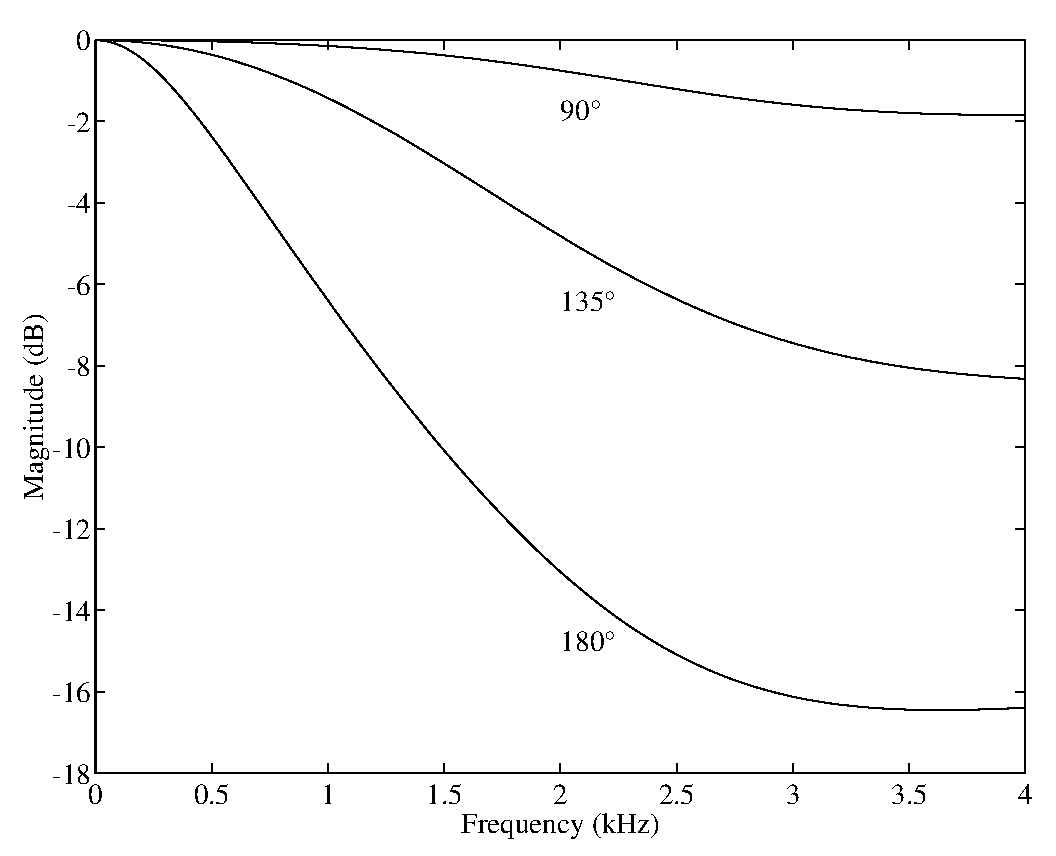
\includegraphics[width=75mm]{figure}}
\caption{{\it Directivity measurement
of a trumpet.}}
\label{fig:figure1}
\end{figure}
\end{verbatim}

\begin{figure}[t]
  \centerline{
    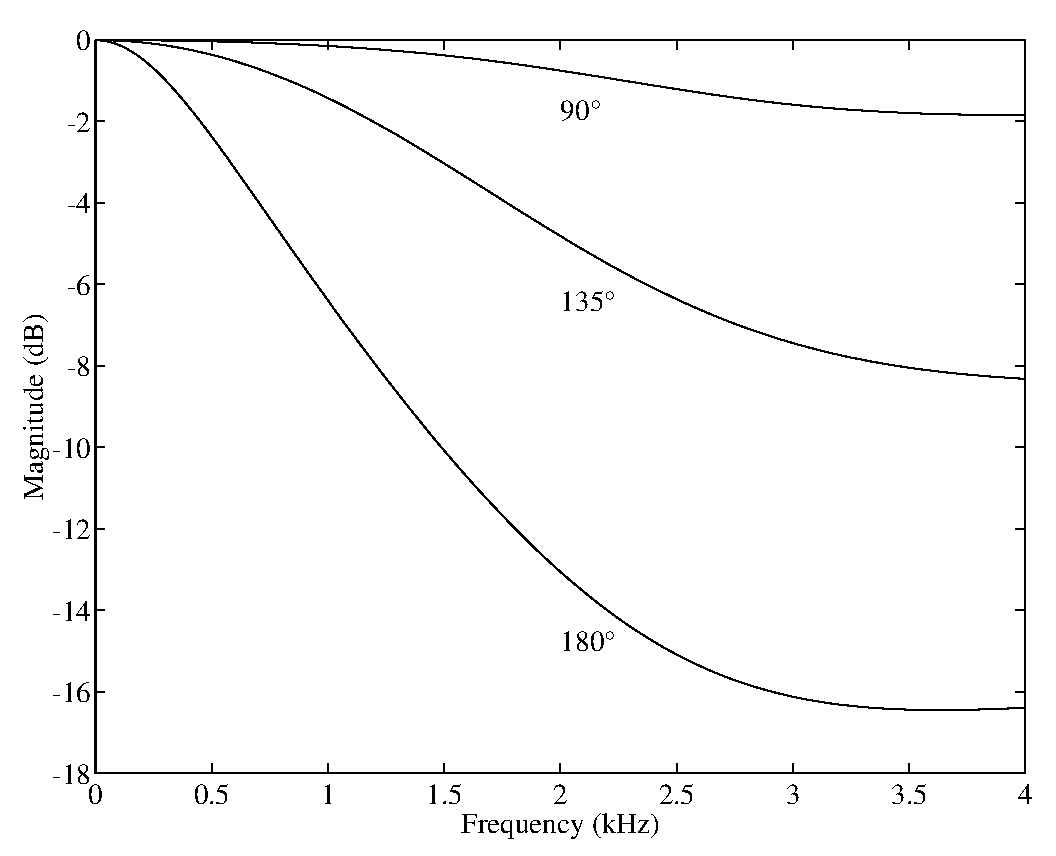
\includegraphics[width=75mm,angle=0]{figure}}
\caption{{\it Directivity measurement of a trumpet.}}
\label{fig:figure1}
\end{figure}

\subsection{Equations}
Equations should be placed on separate lines and numbered:
\begin{equation}
{\bf W}_{WF} = X^{-T} \cdot \textrm{diag} \{ \frac{\sigma_i^2-\eta_i^2}{\sigma_i^2} \} \cdot X^T.
\label{eq:equation1}
\end{equation}


\subsection{References}
List and number all references at the end of the paper. The references
can be numbered in alphabetic order or in order of appearance in the
document. When you add a new reference, insert a bookmark between the
number and the first word of the reference. You will then be able to
refer to the reference in the text by inserting a cross-reference to
the bookmark. This approach guarantees that the numbering will be
correct in the printed document.

In MSWord use ``tools, options, view, bookmarks'' to view the location
of bookmarks. Note that numbers are only updated when you print (or
print preview) the document.

In any case, use reference numbers in square brackets as shown at
the end of this sentence \cite{sps1} \cite{sps3}. The reference
format is the standard IEEE one \cite{sps2}. Check reference
numbering before you submit your paper.

\section{Headings}
Major headings appear in capital letters, bold face if possible,
centered in the column.

\subsection{Sub Headings}
Sub headings appear in capital and lower case, either underlined or in
boldface. They start at the left margin on a separate line.

\subsubsection{Sub-Sub Headings}
Sub-sub headings appear in capital and lower case, indented like a
paragraph and on a separate line and in italic typeface.


\bibliographystyle{IEEEbib}
\bibliography{digitalspeech}

\end{document}
